%%%%%%%%%%%%%%%%%%%%%%%%%%%%%%%%%%%%%%%%%%%%%%%%%%%
\begin{frame}
  \begin{center}
    {\Large Image Classification at FastAI using PyTorch}
    
  \end{center}
  
  \tiny{(Ref: http://course.fast.ai/lessons/lesson1.html)}
\end{frame}

%%%%%%%%%%%%%%%%%%%%%%%%%%%%%%%%%%%%%%%%%%%%%%%%%%%
\begin{frame}[fragile] \frametitle{Download data and Import libraries}
\begin{lstlisting}
!mkdir data && wget http://files.fast.ai/data/dogscats.zip && unzip dogscats.zip -d data/
\end{lstlisting}
Here we import the libraries we need.
\begin{lstlisting}
# This file contains all the main external libs we'll use
from fastai.imports import *
from fastai.transforms import *
from fastai.conv_learner import *
from fastai.model import *
from fastai.dataset import *
from fastai.sgdr import *
from fastai.plots import *
\end{lstlisting}

\end{frame}

%%%%%%%%%%%%%%%%%%%%%%%%%%%%%%%%%%%%%%%%%%%%%%%%%%%
\begin{frame}[fragile] \frametitle{Reading Data}
PATH is the path to your data. sz is the size that the images will be resized to in order to ensure that the training runs quickly. 
\begin{lstlisting}
PATH = "data/dogscats/"
sz=224
torch.cuda.is_available()
>>> True
torch.backends.cudnn.enabled
>>> True

os.listdir(PATH)
os.listdir(f'{PATH}valid') # Listing inside "valid" directory
files = os.listdir(f'{PATH}valid/cats')[:5] # Listing top 4 filenames
files

>>>['cat.6636.jpg',
 'cat.1231.jpg',
 'cat.5769.jpg',
 'cat.1446.jpg',
 'cat.8233.jpg']
\end{lstlisting}

\end{frame}

%%%%%%%%%%%%%%%%%%%%%%%%%%%%%%%%%%%%%%%%%%%%%%%%%%%
\begin{frame}[fragile] \frametitle{Reading Data}
See a sample image
\begin{lstlisting}
img = plt.imread(f'{PATH}valid/cats/{files[0]}')
plt.imshow(img);

img.shape
>>>(374, 500, 3)
\end{lstlisting}
\begin{center}
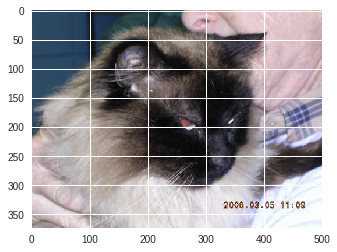
\includegraphics[width=0.5\linewidth,keepaspectratio]{fastai1}
\end{center}
\end{frame}

%%%%%%%%%%%%%%%%%%%%%%%%%%%%%%%%%%%%%%%%%%%%%%%%%%%
\begin{frame}[fragile] \frametitle{Reading Data}
This is what computer stores as image
\begin{lstlisting}
img[:4,:4]
>>> array([[[47, 75, 97],
        [47, 75, 97],
        [47, 75, 97],
        [47, 75, 97]],

       [[47, 75, 97],
        [47, 75, 97],
        [47, 75, 97],
        [47, 75, 97]],

       [[47, 75, 97],
        [47, 75, 97],
        [47, 75, 97],
        [47, 75, 97]],

       [[47, 75, 97],
        [47, 75, 97],
        [47, 75, 97],
        [47, 75, 97]]], dtype=uint8)
\end{lstlisting}

\end{frame}

%%%%%%%%%%%%%%%%%%%%%%%%%%%%%%%%%%%%%%%%%%%%%%%%%%%
\begin{frame}[fragile] \frametitle{Running Pre trained Model}
We will be using the resnet34 model. resnet34 is a version of the model that won the 2015 ImageNet competition. Here is more info on resnet models. We'll be studying them in depth later, but for now we'll focus on using them effectively.
\begin{lstlisting}
arch=resnet34
data = ImageClassifierData.from_paths(PATH, tfms=tfms_from_model(arch, sz),bs=2)
learn = ConvLearner.pretrained(arch, data, precompute=True)
learn.fit(0.01, 3)
\end{lstlisting}
You may get \lstinline|>>> RuntimeError: cuda runtime error (2) : out of memory at /pytorch/torch/lib/THC/generic/THCStorage.cu:58| but nothing much can be done, but restart the kernel and rerun.
\end{frame}

%%%%%%%%%%%%%%%%%%%%%%%%%%%%%%%%%%%%%%%%%%%%%%%%%%%
\begin{frame}[fragile] \frametitle{Results}

\begin{lstlisting}
[0      0.537262   0.677565   0.9]
[1      0.616773   0.346624   0.938 ]
[2      0.54387    0.544023   0.9455]
\end{lstlisting}
First is epoch id, next is loss on training, next is loss on validation and the final is the accuracy number. This would have won the Kaggle Competition at that time (Imagenet 2017, 80\%).
\end{frame}

%%%%%%%%%%%%%%%%%%%%%%%%%%%%%%%%%%%%%%%%%%%%%%%%%%%
\begin{frame}[fragile] \frametitle{Analyzing results: looking at pictures}
As well as looking at the overall metrics, it's also a good idea to look at examples of each of:
\begin{itemize}
\item A few correct labels at random
\item A few incorrect labels at random
\item The most correct labels of each class (ie those with highest probability that are correct)
\item The most incorrect labels of each class (ie those with highest probability that are incorrect)
\item The most uncertain labels (ie those with probability closest to 0.5).
\end{itemize}

\end{frame}

%%%%%%%%%%%%%%%%%%%%%%%%%%%%%%%%%%%%%%%%%%%%%%%%%%%
\begin{frame}[fragile] \frametitle{Results}
We get log probabilities. Need to inverse (exponential) them to get the actual probabilities. 
\begin{lstlisting}
log_preds = learn.predict()
log_preds[:10]
preds = np.argmax(log_preds, axis=1)  # from log probabilities to 0 or 1
probs = np.exp(log_preds[:,1])        # pr(dog)
probs
>>>array([0.08452, 0.11312, 0.009  , ..., 0.65846, 0.79772, 0.68802], dtype=float32)
\end{lstlisting}
Each entries probability of being a DOG is shown above.
\end{frame}


%%%%%%%%%%%%%%%%%%%%%%%%%%%%%%%%%%%%%%%%%%%%%%%%%%%
\begin{frame}[fragile] \frametitle{Utility functions}
Some utility functions to pick images by given characteristics, randomly and plotting.
\begin{lstlisting}
def rand_by_mask(mask): return np.random.choice(np.where(mask)[0], 4, replace=False)
def rand_by_correct(is_correct): return rand_by_mask((preds == data.val_y)==is_correct)

def plot_val_with_title(idxs, title):
    imgs = np.stack([data.val_ds[x][0] for x in idxs])
    title_probs = [probs[x] for x in idxs]
    print(title)
    return plots(data.val_ds.denorm(imgs), rows=1, titles=title_probs)
\end{lstlisting}

\end{frame}

%%%%%%%%%%%%%%%%%%%%%%%%%%%%%%%%%%%%%%%%%%%%%%%%%%%
\begin{frame}[fragile] \frametitle{Utility functions}

\begin{lstlisting}
def plots(ims, figsize=(12,6), rows=1, titles=None):
    f = plt.figure(figsize=figsize)
    for i in range(len(ims)):
        sp = f.add_subplot(rows, len(ims)//rows, i+1)
        sp.axis('Off')
        if titles is not None: sp.set_title(titles[i], fontsize=16)
        plt.imshow(ims[i])
        
def load_img_id(ds, idx): return np.array(PIL.Image.open(PATH+ds.fnames[idx]))

def plot_val_with_title(idxs, title):
    imgs = [load_img_id(data.val_ds,x) for x in idxs]
    title_probs = [probs[x] for x in idxs]
    print(title)
    return plots(imgs, rows=1, titles=title_probs, figsize=(16,8))        
\end{lstlisting}

\end{frame}

%%%%%%%%%%%%%%%%%%%%%%%%%%%%%%%%%%%%%%%%%%%%%%%%%%%
\begin{frame}[fragile] \frametitle{Plots}
A few correct labels at random
\begin{lstlisting}
plot_val_with_title(rand_by_correct(True), "Correctly classified")
\end{lstlisting}
\begin{center}
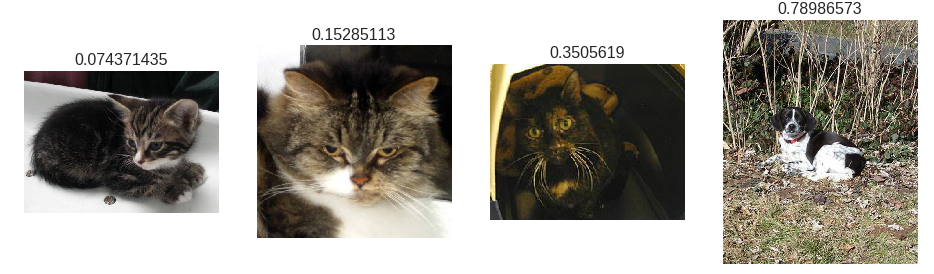
\includegraphics[width=\linewidth,keepaspectratio]{fastai2}
\end{center}
Towards zero values are CATS and towards 1 values are DOGs
\end{frame}

%%%%%%%%%%%%%%%%%%%%%%%%%%%%%%%%%%%%%%%%%%%%%%%%%%%
\begin{frame}[fragile] \frametitle{Plots}
A few incorrect labels at random
\begin{lstlisting}
plot_val_with_title(rand_by_correct(False), "Incorrectly classified")
\end{lstlisting}
\begin{center}
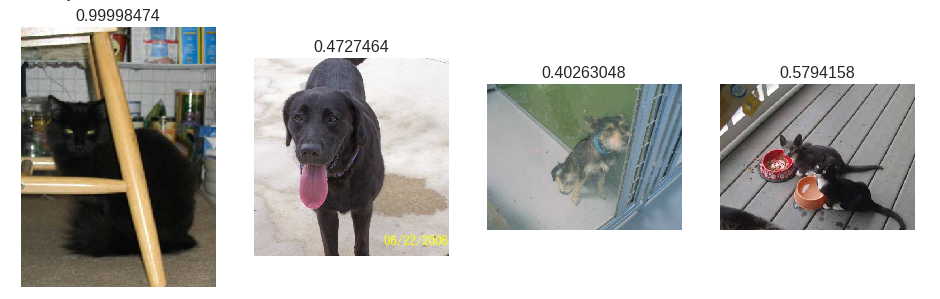
\includegraphics[width=\linewidth,keepaspectratio]{fastai3}
\end{center}
Towards zero values are CATS and towards 1 values are DOGs
\end{frame}

%%%%%%%%%%%%%%%%%%%%%%%%%%%%%%%%%%%%%%%%%%%%%%%%%%%
\begin{frame}[fragile] \frametitle{Utility functions}

\begin{lstlisting}
def most_by_mask(mask, mult):
    idxs = np.where(mask)[0]
    return idxs[np.argsort(mult * probs[idxs])[:4]]

def most_by_correct(y, is_correct): 
    mult = -1 if (y==1)==is_correct else 1
    return most_by_mask(((preds == data.val_y)==is_correct) & (data.val_y == y), mult)
\end{lstlisting}

\end{frame}



%%%%%%%%%%%%%%%%%%%%%%%%%%%%%%%%%%%%%%%%%%%%%%%%%%%
\begin{frame}[fragile] \frametitle{Plots}
Most correct cats
\begin{lstlisting}
plot_val_with_title(most_by_correct(0, True), "Most correct cats")
\end{lstlisting}
\begin{center}
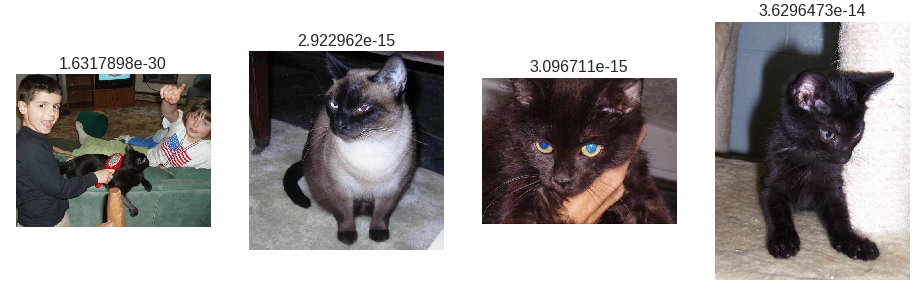
\includegraphics[width=\linewidth,keepaspectratio]{fastai4}
\end{center}
Towards zero values are CATS and towards 1 values are DOGs
\end{frame}

%%%%%%%%%%%%%%%%%%%%%%%%%%%%%%%%%%%%%%%%%%%%%%%%%%%
\begin{frame}[fragile] \frametitle{Plots}
Most correct dogs
\begin{lstlisting}
plot_val_with_title(most_by_correct(1, True), "Most correct dogs")
\end{lstlisting}
\begin{center}
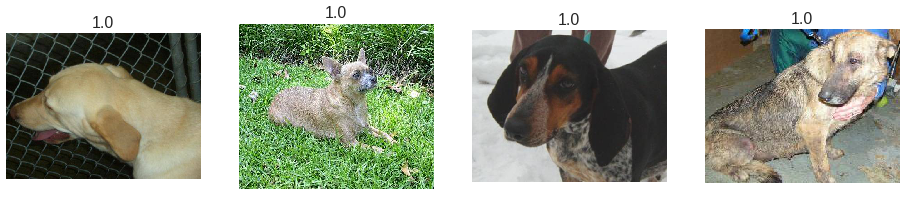
\includegraphics[width=\linewidth,keepaspectratio]{fastai5}
\end{center}
Towards zero values are CATS and towards 1 values are DOGs
\end{frame}

%%%%%%%%%%%%%%%%%%%%%%%%%%%%%%%%%%%%%%%%%%%%%%%%%%%
\begin{frame}[fragile] \frametitle{Plots}
Most incorrect cats
\begin{lstlisting}
plot_val_with_title(most_by_correct(0, False), "Most incorrect cats")
\end{lstlisting}
\begin{center}
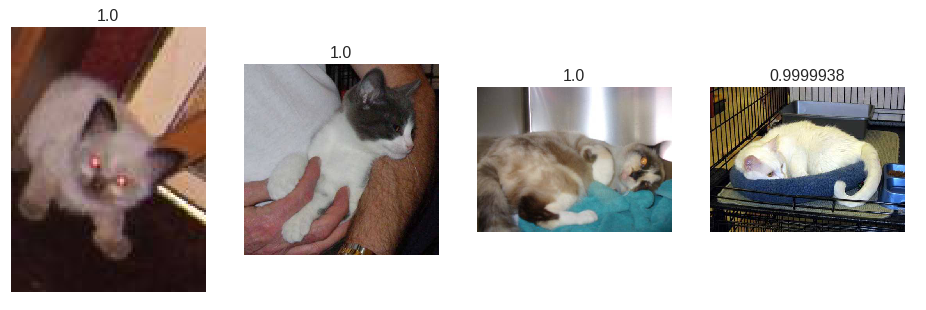
\includegraphics[width=\linewidth,keepaspectratio]{fastai6}
\end{center}
Towards zero values are CATS and towards 1 values are DOGs
\end{frame}

%%%%%%%%%%%%%%%%%%%%%%%%%%%%%%%%%%%%%%%%%%%%%%%%%%%
\begin{frame}[fragile] \frametitle{Plots}
Most incorrect dogs
\begin{lstlisting}
plot_val_with_title(most_by_correct(1, False), "Most incorrect dogs")
\end{lstlisting}
\begin{center}
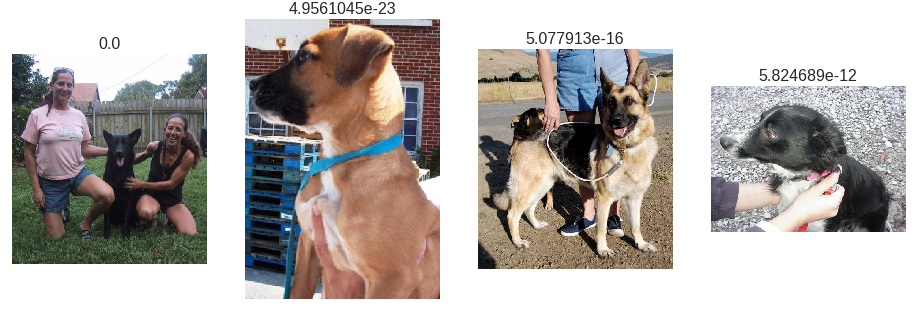
\includegraphics[width=\linewidth,keepaspectratio]{fastai7}
\end{center}
Towards zero values are CATS and towards 1 values are DOGs
\end{frame}

%%%%%%%%%%%%%%%%%%%%%%%%%%%%%%%%%%%%%%%%%%%%%%%%%%%
\begin{frame}[fragile] \frametitle{Plots}
Most uncertain predictions
\begin{lstlisting}
most_uncertain = np.argsort(np.abs(probs -0.5))[:4]
plot_val_with_title(most_uncertain, "Most uncertain predictions")
\end{lstlisting}
\begin{center}
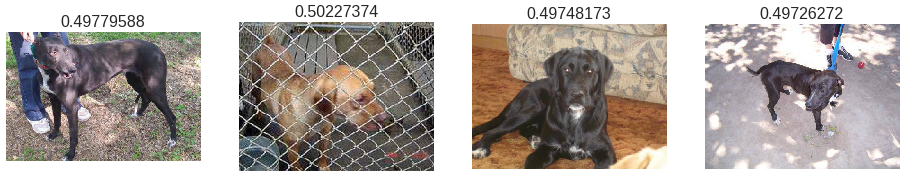
\includegraphics[width=\linewidth,keepaspectratio]{fastai8}
\end{center}
Towards zero values are CATS and towards 1 values are DOGs
\end{frame}

%%%%%%%%%%%%%%%%%%%%%%%%%%%%%%%%%%%%%%%%%%%%%%%%%%%
\begin{frame}[fragile] \frametitle{Improving our model}
Data augmentation
\begin{itemize}
\item If you try training for more epochs, you'll notice that we start to overfit, which means that our model is learning to recognize the specific images in the training set, rather than generalizing such that we also get good results on the validation set. 
\item One way to fix this is to effectively create more data, through data augmentation. 
\item This refers to randomly changing the images in ways that shouldn't impact their interpretation, such as horizontal flipping, zooming, and rotating.
\item We can do this by passing aug\_tfms (augmentation transforms) to tfms\_from\_model, with a list of functions to apply that randomly change the image however we wish.
\end{itemize}

\end{frame}

%%%%%%%%%%%%%%%%%%%%%%%%%%%%%%%%%%%%%%%%%%%%%%%%%%%
\begin{frame}[fragile] \frametitle{Data augmentation}
\begin{lstlisting}
tfms = tfms_from_model(resnet34, sz, aug_tfms=transforms_side_on, max_zoom=1.1)
def get_augs():
    data = ImageClassifierData.from_paths(PATH, bs=2, tfms=tfms, num_workers=1)
    x,_ = next(iter(data.aug_dl))
    return data.trn_ds.denorm(x)[1]
ims = np.stack([get_augs() for i in range(6)])    
plots(ims, rows=2)
\end{lstlisting}
\begin{center}
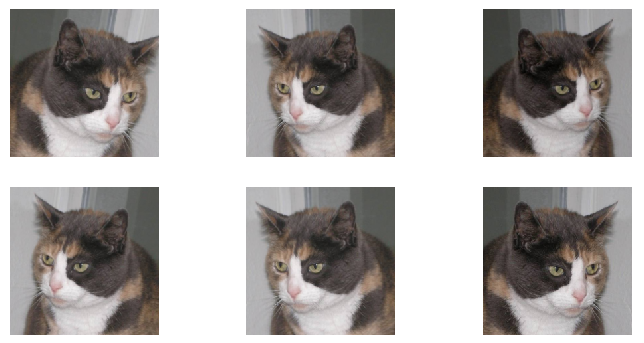
\includegraphics[width=0.8\linewidth,keepaspectratio]{fastai9}
\end{center}
\end{frame}

%%%%%%%%%%%%%%%%%%%%%%%%%%%%%%%%%%%%%%%%%%%%%%%%%%%
\begin{frame}[fragile] \frametitle{Data augmentation}
Let's create a new data object that includes this augmentation in the transforms.
\begin{lstlisting}
data = ImageClassifierData.from_paths(PATH, tfms=tfms)
learn = ConvLearner.pretrained(arch, data, precompute=True)
learn.fit(1e-2, 1)

>>>
epoch      trn_loss   val_loss   accuracy   
    0      0.061966   0.034742   0.988 
\end{lstlisting}
\end{frame}

%%%%%%%%%%%%%%%%%%%%%%%%%%%%%%%%%%%%%%%%%%%%%%%%%%%
\begin{frame}[fragile] \frametitle{Data augmentation}
By default when we create a learner, it sets all but the last layer to frozen. That means that it's still only updating the weights in the last layer when we call fit.
\begin{lstlisting}
learn.precompute=False    
learn.fit(1e-2, 3, cycle_len=1)

>>>
epoch      trn_loss   val_loss   accuracy   
    0      0.046794   0.032046   0.9885 
    1      0.051198   0.030353   0.988
    2      0.056935   0.029544   0.9895    
\end{lstlisting}
\end{frame}


%%%%%%%%%%%%%%%%%%%%%%%%%%%%%%%%%%%%%%%%%%%%%%%%%%%
\begin{frame}[fragile] \frametitle{Test Time Augmentation (TTA)}
TTA simply makes predictions not just on the images in your validation set, but also makes predictions on a number of randomly augmented versions of them too
\begin{lstlisting}
log_preds,y = learn.TTA()
probs = np.mean(np.exp(log_preds),0)
accuracy(log_preds, y)
>>>0.995
\end{lstlisting}
\end{frame}

%%%%%%%%%%%%%%%%%%%%%%%%%%%%%%%%%%%%%%%%%%%%%%%%%%%
\begin{frame}[fragile] \frametitle{Review: easy steps to train a world-class image classifier}
\begin{itemize}
\item Enable data augmentation, and precompute=True
\item Train last layer from precomputed activations for 1-2 epochs
\item Train last layer with data augmentation (i.e. precompute=False) for 2-3 epochs with cycle\_len=1
\item Unfreeze all layers
\item Set earlier layers to 3x-10x lower learning rate than next higher layer
\item Train full network with cycle\_mult=2 until over-fitting
\end{itemize}

\end{frame}